65. Возможны два случая расположения точек $A$ и $B$ на стороне $PC.$ В первом случае точки расположены в порядке $P,\ A,\ B,\ C.$
\begin{figure}[ht!]
\center{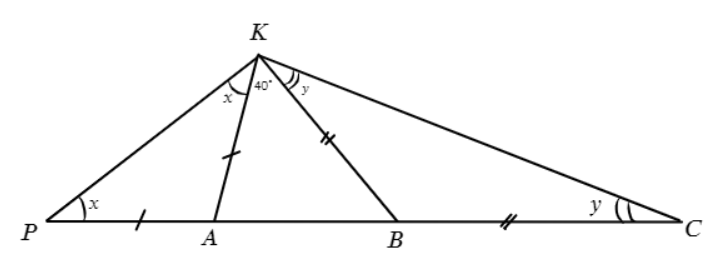
\includegraphics[scale=0.35]{g65-1.png}}
\end{figure}\\
Треугольники $PAK$ и $CBK$ являются равнобедренными, обозначим их углы при основании буквами $x$ и $y.$ Тогда из треугольника $PKC$ имеем $2x+2y+40^\circ=180^\circ,\ x+y=70^\circ.$ Таким образом, $\angle PKC=x+y+40^\circ=70^\circ+40^\circ=110^\circ.$\\
Во втором случае точки расположены в порядке $P,\ B,\ A,\ C.$
\begin{figure}[ht!]
\center{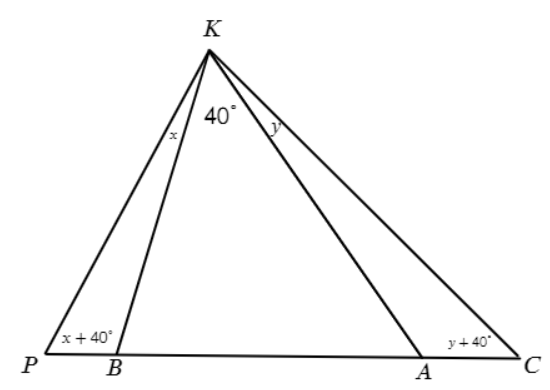
\includegraphics[scale=0.35]{g65-2.png}}
\end{figure}\\
В этом случае обозначим $\angle PKB=x,\ \angle AKC=y,$ тогда $\angle P=x+40^\circ,\ \angle C=y+40^\circ.$ Из треугольника $PKC$ имеем $x+40^\circ+y+40^\circ+x+y+40^\circ=180^\circ,\ x+y=30^\circ.$ Таким образом, $\angle PKC=x+y+40^\circ=30^\circ+40^\circ=70^\circ.$\\
